\makesection{Base di partenza}

\begin{frame}{}
    \begin{wrapfigure}{r}{0.75\textwidth}
    \centering
    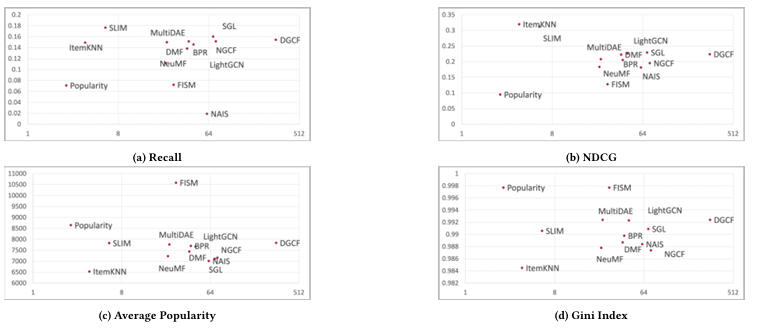
\includegraphics[width=0.75\textwidth]{images/risultati-valutazione.png}
    \caption{Trade-off tra emissioni e performance con dataset Mind}
\end{wrapfigure}

In questo ambito sono stati già svolti diversi esperimenti che mostrano come spesso algoritmi più semplici riescono ad avere delle performance molto simili (se non migliori) a modelli più complessi, ma con un impatto ambientale decisamente minore.
\end{frame}

\begin{frame}{}
    Una strategia comune per calcolare il CO$_2$eq è quella di moltiplicare tra loro il \textbf{carbon intensity(CI)} e l'\textbf{energia consumata(PC)} dall'attività (nel nostro caso l'esecuzione di algoritmi).



    \begin{equation*}
        \textit{emission} = \textit{CI}  \cdot \textit{PC}
    \end{equation*}
    
    \noindent In particolare i valori di CI dipendono dalle diverse fonti di energia utilizzate durante la computazione 
    (es. energia solare, energia eolica, etc.). Se \textit{s} è la fonte di energia,  \textit{e$_s$} sono le emissioni per KW/h di energia e \textit{p$_s$}  è la percentuale di energia prodotta dalla fonte s, allora il CI è dato da:
    \begin{equation*}
        \textit{CI} = \sum_{s \in S} \textit{e$_s$} \cdot \textit{p$_s$}
    \end{equation*}
\end{frame}

\begin{frame}{}
    \begin{wrapfigure}{r}{0.4\textwidth}
        \centering
        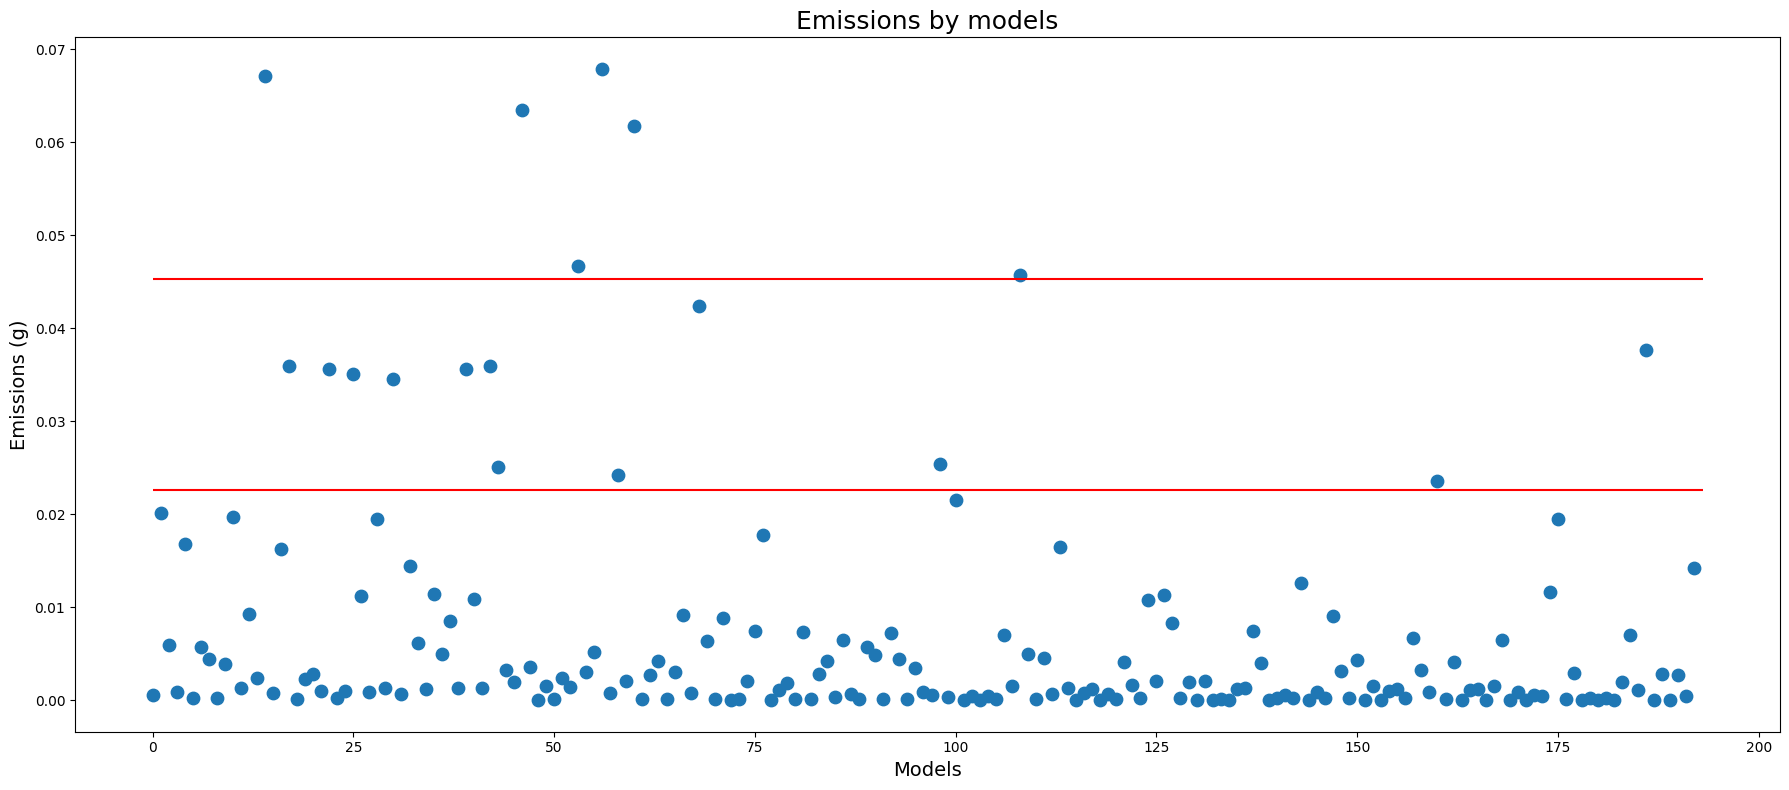
\includegraphics[width=0.4\textwidth]{images/situazione-attuale.png}
        \caption{Dataset iniziale}
    \end{wrapfigure}
    
    Qui possiamo notare la distribuzione delle emissioni prodotte dagli esperimenti iniziali.
    Il dataset del regressore è descritto dalle seguenti features di input:
    \begin{itemize}
        \small
        \item \textbf{n\_users}: numero di utenti
        \item \textbf{n\_items}: numero di item
        \item \textbf{n\_inter}: numero di interazioni
        \item \textbf{sparsity}: sparsità del dataset
        \item \textbf{kg\_entities}: numero di entità nel knowledge graph
        \item \textbf{kg\_relations}: numero di relazioni nel knowledge graph
        \item \textbf{kg\_triples}: numero di triple nel knowledge graph
        \item \textbf{kg\_items}: numero di item nel knowledge graph
        \item \textbf{cpu\_cores}: numero di core della CPU
        \item \textbf{ram\_size}: quantità di RAM
        \item \textbf{is\_gpu}: presenza di una GPU
        \item \textbf{model\_name}: nome del modello
        \item \textbf{model\_type}: tipo di modello
    \end{itemize}
\end{frame}

\begin{frame}{Regressore - Introduzione}
Sono stati utilizzati diversi modelli di regressione per prevedere le emissioni prodotte da un modello di raccomandazione in base alle features di input. I modelli utilizzati sono:
\begin{itemize}
    \item \textbf{Random Forest} : sono modelli di regressione basati su alberi deci
    sionali. Vengono costruiti su più alberi decisionali che combinano le loro previsioni per ottenere una previsione
     pi` u accurata e stabile
    \item \textbf{Decision Tree}: sono modelli di regressione basati su alberi decisionali
    \item \textbf{AdaBoost}:  L’AdaBoost Regressor è un modello basato sull’algoritmo di boosting AdaBoost.
    Questo algoritmo costruisce un modello di previsione combinando pi` u modelli di previsione più deboli.
    \item \textbf{SVG}: è un algoritmo che estende il concetto di Support Vector Machine (SVM) al caso della regressione
\end{itemize}
\end{frame}
    


\begin{frame}{Regressore - Analisi dei risultati}
    \begin{wrapfigure}{r}{0.35\textwidth}
    \centering
    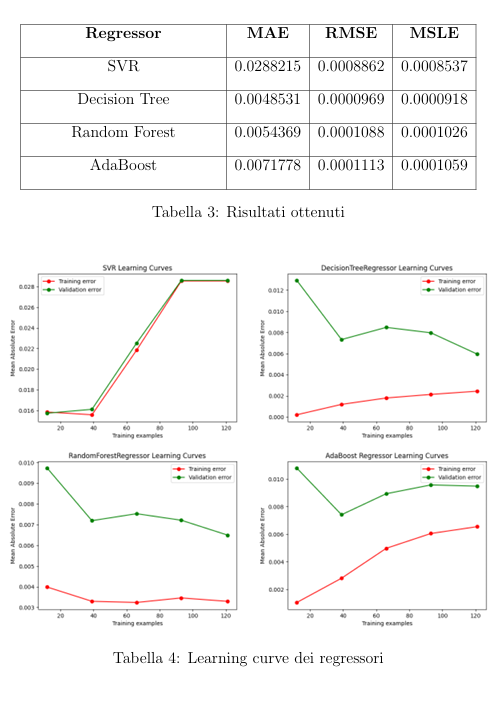
\includegraphics[width=0.35\textwidth]{images/RegressorePrecedente.png}
    \caption{Risultati}
\end{wrapfigure}

E' stato utilizzato uno split del 70\% per il training e del 30\% per il testing.
Il dataset sembra essere troppo piccolo per poter generalizzare bene i modelli. Inoltre, il dataset è molto sbilanciato, con pochi valori per ogni feature. Per i risultati attuali, il Decision Tree Regressor è il modello migliore
\end{frame}
